% CUSTOM TEMPLATE FOR SOLUTIONS STARTS
\documentclass[answers]{exam}
 
 \usepackage{graphicx}
 \usepackage{float}
 \usepackage{amsmath}
 \usepackage{amsfonts}
 \usepackage{framed}
 \usepackage{algorithmicx}
 \usepackage{algpseudocode}
 \newcommand{\ans}[1]{\begin{framed}{\textbf{Answer:} #1}\end{framed}}
 \newcommand{\sol}{\uplevel{\textsc{Solution:}}}
 \newenvironment{answer}{%
     \renewcommand{\solutiontitle}{\noindent\textbf{Answer:}\enspace}
     \begin{solution}
     }{%
     \end{solution}
     \renewcommand{\solutiontitle}{\noindent\textbf{Solution:}\enspace}
 }
% CUSTOM TEMPLATE FOR SOLUTIONS ENDS

% First we setup the header and footer
\pagestyle{headandfoot}
\runningheadrule
\runningfootrule
\header{COL351: Analysis and Design of Algorithms (CSE, IITD, Semester-I-2020-21)}{}{Minor Exam}
\footer{}{\thepage  \, of \numpages}{}
 
% We want the points for each question displayed on the left
%\pointname{points}
%\pointsinmargin
 
% Automatically total the points - make sure to compile TWICE
\addpoints
 
\begin{document}


\vspace{0.1in}


\vspace{0.1in}
% Some general text together with number of questions and total points possible
There are \numquestions\, questions for a total of \numpoints\, points.
\vspace{0.1in}
\hrule
 \vspace{0.2in}
\begin{questions}
 
\question[5] 

    \begin{parts}

        \part For any $n>3$ and any directed graph $G$ with $n$ vertices, if the number of edges in $G$ is $n$, then the number of strongly connected components of $G$ is strictly less than nnn.
        \begin{answer}
        False
        \end{answer}

        \part How many SCCs does this graph have?
            \begin{center}
                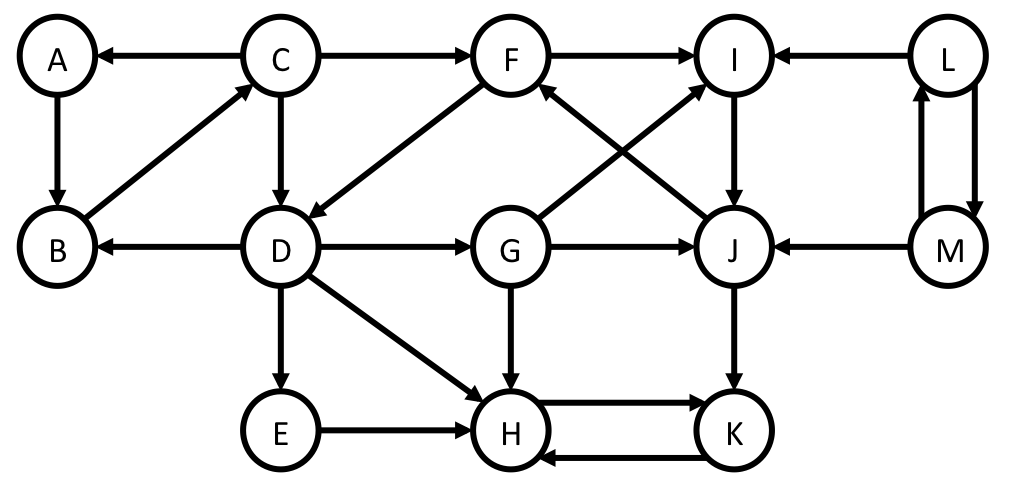
\includegraphics[scale=0.25]{minor/scc_minor.png}
            \end{center}
        \begin{answer}
            4
        \end{answer}

        \part Give all the vertices that are in the strongly connected component that contains the vertex $D$ in the graph given.
        \begin{answer}
            $A, B, C, D, F, G, I, J$
        \end{answer}

        \part For any directed acyclic graph $G$ that has a unique source vertex, this source vertex is the first vertex in every topological ordering of vertices of $G$.
        \begin{answer}
            True
        \end{answer}

        \part Let $G$ be an undirected graph on $n$ nodes where $n$ is an even number. If every node of $G$ has degree $\geq n/2$, then $G$ is strongly connected.
        \begin{answer}
            True
        \end{answer}

    \end{parts}

\question[7]

You are given directed acyclic graph $G = (V, E)$ and you want to determine if $G$ has a unique topological ordering (i.e., whether there is exactly one topological ordering of the vertices).

(For example, the DAG on the left  does not have a unique topological ordering since both $a, b, c, d$ and $a, c, b, d$ are valid topological orderings. However, the DAG on the right has a unique
    topological ordering $a, c, b, d$.)

    \begin{center}
        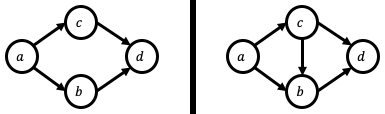
\includegraphics[scale=0.5]{minor/graph.png}
    \end{center}

Assume that the DAG is given in adjacency list representation. Design an algorithm for this problem. Your algorithm should output ``yes" if $G$ has a unique topological ordering and ``no" otherwise. Give running time analysis and proof of correctness for your algorithm.

[Points distribution: Algorithm (3 points), proof of correctness (3 points), running time analysis (1 points)]

\begin{solution}
    \textbf{Algorithm:}

    \begin{algorithmic}
        \Function{HasUniqueTopologicalOrder}{$G = (V, E)$}
            \If{$|V| = 0$}
                \State output ``yes"
            \EndIf
            \State initialize array $in[1\ldots |V|]$ with 0s
            \For{$v \in V$}
                \For{$(v, u) \in E$}
                    \State $in[u] := in[u] + 1$
                \EndFor
            \EndFor
            \State $order :=$ \Call{Linearize}{$G$}
            \State $sources := 0$
            \For{$v \in V$}
                \If{$in[v] = 0$} 
                    \State $sources := sources + 1$
                \EndIf
            \EndFor
            \If{$sources > 1$}
                \State output ``no"
                \State \Return
            \EndIf
            \For{$i \in 1..|V|$}:
                \State $sources := sources - 1$
                \State $v := order[i]$
                \For{$(v, u) \in E$}
                    \State $in[u] := in[u] - 1$
                    \If{$in[u] = 0$}
                        \State $sources := sources + 1$
                    \EndIf
                \EndFor
            \EndFor
            \If{$sources > 1$}
                \State output ``no"
                \State \Return
            \EndIf
            \State output ``yes"
            \State \Return
        \EndFunction
    \end{algorithmic}

    \textbf{Proof of correctness:}

Note that the empty graph vacuously has a unique topological ordering. Henceforth we assume $G$ is non-empty.

Firstly we claim that after the first loop, $in[v]$ contains the indegree of vertex $v$.

    \textit{Proof}: We iterate over all possible edges in the first loop (all edges have been covered since each edge has a starting vertex, which is iterated over since it is in $V$, and they are
    covered exactly once since no edge has two starting vertices), and for each edge with the ending vertex as $v$, we increment $in[v]$. This implies, given the initial value of $in[v]$ to be $0$,
    that $in[v]$ finally contains the number of incoming edges to $v$, which is the indegree of $v$.

Then we claim that after the second loop, $sources$ contains the number of sources of the graph.

    \textit{Proof:} We iterate over all vertices and increment $sources$ by 1 iff the indegree of the vertex is 0, and thus $sources$ is precisely the number of vertices with indegree 0, which are precisely all the sources of the graph by definition.

Note that if for a graph, there are at least 2 sources, say $u, v$, then we can come up with a topological order with the first two vertices as $u, v$ and $v, u$ (as both are sources) and the rest of the order being the same, which implies that there are at least 2 topological orderings of the graph.

Hence for a graph to have a unique topological ordering, it is necessary that there is exactly one source.

Now we claim that if we remove the unique source from $G$ and the remaining graph $G'$ also has a unique topological ordering, then $G$ also has a unique topological ordering, and vice versa.

\textit{Proof:}

(forward direction) Suppose not. Then there are at least 2 topological orderings of $G$, and since it has a unique source, the first element in each ordering is the unique source. If
we remove the first element of both the orderings, then we claim that the remaining orderings are topological orderings for $G'$, which will give a contradiction. To prove this claim, we do the following.
Note that by the definition of topological ordering, for any edge $(u, v)$ in $G, u$ is to the left of $v$ in the ordering. Consider any edge $(u, v)$ in $G'$. Since $(u, v)$ is in G, and $u$ is not
the source of G, both $u$ and $v$ are in the new ordering and $u$ is to the left of $v$ in the new ordering. Thus the new ordering (which is obtained by removing the unique source of $G$) is also a
valid topological ordering for $G'$ which proves the subclaim. As we had noted earlier, this implies that $G'$ has two distinct topological orderings if we remove the source of $G$ from the two
distinct topological orderings of $G$, and this is a contradiction. Hence there can only be at most 1 topological ordering of $G$, and since $G$ is a DAG, it has a unique topological ordering.

(backward direction) If $G'$ has at least two topological orderings, by an argument similar to the above, we can see that if we insert the unique source in the beginning of any ordering for $G'$ we
come up with a valid topological order of $G$, so we get at least two topological orderings of $G$, which is a contradiction.

Now we claim that after the $i^\mathrm{th}$ iteration in the final loop, either we have returned or $in[]$ contains the indegrees of all vertices in the graph $G_i$ obtained by removing vertices $1,
\dots, i$ from $G$.

\textit{Proof:} Induction on $i$.

Base case: $i = 0$: this is vacuously true.

Inductive hypothesis: 
$P(i)$: after the ith iteration in the final loop, either we have returned or $in[]$ contains the indegrees of all vertices in the graph $G_i$.

Inductive step:
Suppose $P(i)$ is true. We need to show $P(i + 1)$.

If we have returned already, we are done. Otherwise, note that $in[v]$ = indegree of $v$ in the graph $G_i$ before this iteration. When we remove the vertex $order[i]$, note that it is a source of the
graph since the remaining ordering is a valid topological ordering of $G_{i + 1}$. Hence all edges that need to be removed are those emanating from $order[i]$, and thus for each neighbour $u$ of
$order[i]$ (which is to its right in the topological ordering since it is a source), we decrement $in[u]$. After we have done this, we can see that this preserves the property that $in[u]$ has the
indegree of $u$ in $G_{i + 1}$ since either it is adjacent to $order[i]$ or it isn't, and in the case it is, we decrement it by 1, and in the case it isn't, we don't. Hence $P(i + 1)$ is true, and the induction is complete.

Now we claim that after the $i^\mathrm{th}$ iteration in the final loop, either we have returned or sources contains the number of sources in $G_i$.

\textit{Proof}: Induction on $i$.

Base case: $i = 0$: follows from the previous claim regarding sources.

Inductive hypothesis: after the $i^\mathrm{th}$ iteration in the final loop, either we have returned or sources contains the number of sources in $G_i$.

Inductive step:

Suppose $P(i)$ is true. We need to show $P(i + 1)$. 
Note that when we remove $order[i]$ we need to decrement sources by $1$ since $order[i]$ was a source in $G_i$ but is not a vertex in $G_{i + 1}$. Now we increment it by 1 for each vertex whose new
indegree is 0 after removing this from the graph (the validity of new indegree follows from the previous claim), i.e., each new source in the graph. Hence sources is the number of the sources in $G_{i
+ 1}$ and $P(i + 1)$ is proved.

Now we show that if we output ``no", G doesn't have a unique topological ordering, and if we output ``yes", then G has a unique topological ordering.

\textit{Proof:}

Suppose we output ``no". Then after some $i^\mathrm{th}$ iteration, the number of sources is $> 1$ (the iteration where we return). This implies that $G_{i}$ has at least 2 topological orderings.
Now we show using induction that G has at least 2 topological orderings.

Proof:

Inductive hypothesis: $P(k):$ $G_{i - k}$ has at least 2 topological orderings for $k \le i$.

Base case: for $k = 0$, this is true by assumption.

Inductive step: suppose $P(k)$ is true for some $k < i$, we need to show $P(k + 1)$ is true.

Note that $G_{i - k}$ has at least 2 topological orderings, so $G_{i - k - 1}$ also has at least 2 topological orderings, by the application of the claim proved above (the contrapositive of the
backward direction). Hence $P(k + 1)$ is true, which completes the induction.

Thus $P(i)$ is true, and this implies that $G$, which is $G_0$, has at least two topological orderings.

Now suppose we output ``yes". This means that at all iterations, the number of sources is at most $1$.

We show using induction that $G$ has exactly 1 topological ordering.

Proof:

Induction hypothesis: $P(k):$ $G_{n - k}$ has exactly 1 topological ordering for $k \le i$.

Base case: for $k = 0, 1$, this is true since a graph with 0 or 1 vertices has exactly 1 topological ordering.

Inductive step: suppose $P(k)$ is true for some $0 < k < n$, we need to show $P(k + 1)$ is true.

Note that by the claim above, if $G_{n - k}$ has exactly 1 topological ordering and $G_{n - k - 1}$ has exactly one source, then $G_{n - k - 1}$ also has exactly 1 topological ordering. However, using
the inductive hypothesis, $G_{n - k}$ has exactly 1 topological ordering and $G_{n - k - 1}$ has exactly one source since we never returned ``no" (which means $sources \le 1$ and $sources \neq 0$
since the graph is non empty as $k > 0$). Thus $P(k + 1)$ is true and we are done.
In particular, $G_0$ which is $G$ also has a unique topological ordering, so we are done.

Therefore, our output is correct and we are done.

\textbf{Running time analysis:}
Initialising takes $O(V)$ time, the first loop takes $O(V + E)$ time due to iteration over the adjacency list, the second loop takes $O(V)$ time, linearizing takes $O(V + E)$ time, and the final loop
takes $O(V + E)$ time due to iterating over the adjacency list and doing $O(1)$ work in the inside and the outside loop. Thus the overall complexity is $O(V + E)$ which is linear.
\end{solution}

\question[8]

There are $n$ cookies with $s_1 \geq s_2 \geq ... \geq s_n$ and there are $n$ cookie monsters with cookie size requirements $r_1 \geq r_2 \geq ... \geq r_n$. The problem is to distribute the $n$ cookies to the cookie monsters such that:

    \begin{enumerate}
        \item every cookie monster gets exactly one cookie, and
        \item the number of satisfied cookie monsters is maximised. A cookie monster is satisfied iff it gets a cookie that has size at least its cookie size requirement.
    \end{enumerate}

Design an algorithm for this problem. The output can be given as a set of tuples $\{(i_1, j_1), ..., (i_n, j_n)\}$. This means that, as per this distribution, cookie number $i_t$ should be given to
monster number $j_t$ for all $t \in \{1, 2, ..., n\}$.

(For example, consider an input with two cookies with size $5, 3$ and two cookie monsters with size requirements $4, 2$. For the assignment $\{(1, 2), (2, 1)\}$, the number of satisfied cookie
monsters is one. For the assignment $\{(1, 1), (2, 2)\}$, the number of satisfied cookie monsters is two.)

Here is a greedy strategy for this problem.

    Greedy strategy: Give the cookie number $1$ to the first cookie monster (in order $1, ..., n$) that is satisfied by this cookie. Let $j$ be this cookie monster. That is, $s_1 \geq
    r_j$ and $s_1 < r_1, s_1 < r_2, ..., s_{j-1} < r_{j-1}$. Then recursively distribute cookies $2, ..., n$ to cookie monsters $j+1, ..., n$. At the end of this process, arbitrarily distribute the remaining cookies to the remaining monsters.

\begin{parts}
    \part Prove correctness of the above greedy strategy.
    \begin{solution}

We prove this using an exchange argument. 

Define $value(OA)$ = number of satisfied monsters in a given assignment $OA.$

Exchange lemma:

        If there exists a monster which can be satisfied by the first cookie, for any valid assignment of cookies $OA,$ there is an assignment of cookies $OA'$ such that the first cookie is given to
        the monster with the largest requirement which can be satisfied using it, and $value(OA') \ge value(OA).$

        \textit{Proof:}

        $OA$ satisfies the constraints by definition. Consider the first cookie $c$. Suppose it has been assigned to a monster $m$. Suppose the monster with the largest requirement which can be
        satisfied using it is $M$, and $M$ is assigned $C$. Consider the solution $OA' = OA - \{(c, m), (C, M)\} \cup \{(c, M), (C, m)\}$. Note that $M$ is satisfied by $c$ as per the definition of
        $M$. $OA'$ meets constraints since exchanging still upholds the property that the cookie-to-cookie-monster mapping is a bijection. Now we make cases as follows:

        \begin{enumerate}
            \item
                $M$ is satisfied by $C$ and $m$ is satisfied by $c$. 
                $m$ is also satisfied by $C$ as the requirement of $m$ is $<$ requirement of $M$, so no change in number of satisfied monsters.
            \item $M$ is not satisfied by $C$ and $m$ is satisfied by $c$.
                $M$ is satisfied by $c$ and $m$ may or may not be satisfied by $C$, so the number of satisfied monsters remains the same or increases by 1.
            \item $m$ is not satisfied by $c$. 
                This case isn't possible since requirement of $m$ can't exceed that of $M$ by definition of $M$, and $M$ is satisfied by $c$, so $m$ must be satisfied by $c$ as well.
        \end{enumerate}
Hence by the analysis above, we see that $OA'$ is at least better than $OA$ and we have proved the exchange lemma.

Now we show using induction on the number of cookies that the greedy algorithm gives an optimal solution.

Base case:

For the number of cookies being 0 or 1, we are done because there can be exactly 1 assignment for each of these cases.

Induction step:

Now suppose number of cookies is $c > 1$.

If there is no monster which can be satisfied by the largest cookie, we can see that no monster can be satisfied by any cookie, so an optimal solution in this case would be an arbitrary assignment, which is what the greedy algorithm does in this case.

Now suppose the set of cookie monsters which can be satisfied by the largest cookie $c$ is non-empty, and hence the cookie monster with the largest requirement in this set exists, say $M$.
Let the greedy solution to this problem be $GA$.

Consider any solution $OA$ to this problem, and let $OA'$ be defined as in the exchange lemma.
Then $OA' = (c, M) \cup $(solution on the instance where cookie $c$ and monster $M$ are removed, say $OS$), and by the exchange lemma, we have $value(OA') \ge value(OA)$.

Let $GS$ be the greedy solution corresponding to the instance where cookie $c$ and monster $M$ are removed. By the inductive hypothesis, we have $value(GS) \ge value(OS)$. Then we have, from the above, that 

        $$value(GA) = 1 + value(GS) \ge 1 + value(OS) = value(OA') \ge value(OA)$$

Hence, we have shown that in any case, value of the greedy solution is greater than or equal to the value of any other solution for $c$ cookies. 
Specialising to the case where the ``any other solution" is an optimal solution $Opt$, we see that the value of the greedy solution (say $Greedy$) is greater than or equal to $value(Opt)$. Since
        $Opt$ is optimal, $value(Greedy)$ can not exceed $value(Opt)$, and thus must be equal. Thus $Greedy$ is optimal for $c$ cookies, and our induction is complete.

Now, taking the number of cookies to be $n$ and the problem instance to be the one given to us, using the result above, we conclude that the greedy solution is optimal for our instance as well.
    \end{solution}
    \part Give an efficient algorithm implementing the above strategy, and give a running time analysis for your algorithm.
    \begin{solution}

        \begin{algorithmic}
            \Function{Solve}{$n, s, r$}
                \State $j := 1$
                \State $stop := n + 1$
                \State $unsatisfied := $ empty linked list
                \State $assignment := $ empty linked list
                \For{$i \in \{1, \ldots, n\}$}
                    \While{$j \le n \land r[j] > s[i]$}
                        \State insert $j$ into $unsatisfied$
                        \State $j := j + 1$
                    \EndWhile
                    \If{$j \le n$}
                        \State insert $(i, j)$ into $assignment$
                        \State $j := j + 1$
                    \Else
                        \State $stop := i$
                        \State break
                    \EndIf
                \EndFor
                \While{$stop \le n$}
                    \State pop $j$ from $unsatisfied$
                    \State insert $(stop, j)$ into $assignment$
                    \State $stop := stop + 1$
                \EndWhile
                \State \Return $assignment$
            \EndFunction
        \end{algorithmic}

        \textbf{Running time analysis:}

The first four lines of the function take $O(1)$ time.
        Now consider the loop. For each iteration, let $j_{i_{old}}$ and $j_{i_{new}}$ be the values of $j$ before and after this iteration. The inner loop takes time $O(j_{i_{new}} - j_{i_{old}})$ and the outer
        loop takes a constant amount of extra time apart from this time. Thus the total time taken is $O(i_{final} + j_{i_{final, new}} - 1))$ where $i_{final} (= stop)$ is the value of $i$ where we break
        the loop (or $n$ if the loop ends without any break from our side). Since $i$ and $j$ can be at most $n + 1$, this takes time $O(n)$. The final loop which does assignment takes $O(n)$ time
        (more precisely $O(n - j_{i_{final, new}})$ time) since it takes $O(1)$ time inside each iteration.
Thus the overall complexity is $O(n)$, which is linear.
    \end{solution}
\end{parts}

\end{questions}
\end{document}

